\documentclass[12pt,a4paper]{article}

% Packages
\usepackage[margin=1in]{geometry}
\usepackage{titlesec}
\usepackage{booktabs}
\usepackage{array}
\usepackage{tabularx}
\usepackage{xcolor}
\usepackage{hyperref}
\usepackage{enumitem}
\usepackage{parskip}
\usepackage{graphicx}
\usepackage{fancyhdr}
\setlength{\headheight}{14.5pt}
\usepackage{amsmath}
\usepackage{float}

% Colors
\definecolor{headingblue}{RGB}{31, 73, 125}
\definecolor{accentblue}{RGB}{70, 130, 180}
\definecolor{lightgray}{RGB}{245, 245, 245}
\definecolor{tablehead}{RGB}{31, 73, 125}
\definecolor{nfrcolor}{RGB}{0, 102, 153}

% Title formatting
\titleformat{\section}{\large\bfseries\color{headingblue}}{}{0em}{}[\titlerule]
\titleformat{\subsection}{\normalsize\bfseries\color{accentblue}}{}{0em}{}
\titleformat{\subsubsection}{\normalsize\bfseries}{}{0em}{}

% Header/Footer
\pagestyle{fancy}
\fancyhf{}
\rhead{\textcolor{gray}{\small DocPilot --- Task 3}}
\lhead{\textcolor{gray}{\small S26CS6.401 Software Engineering}}
\cfoot{\thepage}
\renewcommand{\headrulewidth}{0.4pt}

% Hyperref setup
\hypersetup{
    colorlinks=true,
    linkcolor=headingblue,
    urlcolor=accentblue
}

% Custom table column
\newcolumntype{L}[1]{>{\raggedright\arraybackslash}p{#1}}



\begin{document}

% Title Page
\begin{titlepage}
    \centering
    \vspace*{2cm}
    {\Huge\bfseries\color{headingblue} DocPilot\par}
    \vspace{0.5cm}
    {\Large A Copilot-Inspired Multi-Model Document Intelligence Platform\par}
    \vspace{1.5cm}
    {\large\bfseries Task 3: Architectural Tactics and Patterns\par}
    \vspace{0.5cm}
    {\large S26CS6.401 --- Software Engineering\par}
    \vspace{1cm}
    \rule{0.5\textwidth}{0.4pt}\\[0.5cm]
    {\large Team No.\ 38\par}
    \vspace{0.5cm}
    {\normalsize Domain: Productivity\par}
    \vfill
    {\normalsize \today\par}
\end{titlepage}

\tableofcontents
\newpage

% ============================================================
\section{Task 3: Architectural Tactics and Patterns}
% ============================================================

Architectural tactics are design decisions that directly influence a system's ability to achieve a
desired quality attribute response. As defined in course literature, a tactic is a characterization
of an architectural decision targeted at a specific quality concern. For DocPilot, the tactics below
were selected to directly address the NFRs established in Task~1 and the constraints arising from a
multi-model, RAG-based document intelligence pipeline.

% ============================================================
\subsection{3.1 Architectural Tactics}
% ============================================================

DocPilot employs five architectural tactics, each mapped to one or more non-functional requirements.
Each tactic is described using the quality-scenario structure (Source, Stimulus, Artifact,
Environment, Response, Response Measure) consistent with the Len Bass quality-scenario model.

% ----------------------------------------------------------
\subsubsection{Tactic 1 --- Passive Redundancy / Spare (Availability)}
% ----------------------------------------------------------

\paragraph{Quality Attribute:} Availability

\paragraph{NFR Addressed:} NFR6 --- Model fallback must initiate within 2 seconds.

\paragraph{Description.}
When a user submits a query and the primary LLM provider (e.g.\ GPT-4o) is unavailable---either
due to a service outage, rate-limit exhaustion, or network timeout---the system automatically
switches to a pre-configured fallback model (e.g.\ Claude 3 or Gemini 1.5) without requiring any
user intervention. This is realized through the \textit{Chain of Responsibility} pattern in the
\texttt{ModelGateway}, where each handler in the chain attempts to fulfill the request and passes it
downstream on failure.

The tactic falls under the \textbf{Fault Recovery} branch of Availability Tactics (specifically,
\textit{Spare/Passive Redundancy}): a set of backup models is kept warm and configured, ready to
receive traffic if the primary fails.

\paragraph{Quality Scenario.}

\begin{center}
\begin{tabular}{@{}L{3.5cm}L{9cm}@{}}
\toprule
\textbf{Element} & \textbf{Value} \\
\midrule
Source & External (LLM provider infrastructure) \\
Stimulus & Primary model returns a timeout or 503 error (omission fault) \\
Artifact & \texttt{ModelGateway} --- Chain of Responsibility handler chain \\
Environment & Normal operation (user-initiated Q\&A or editing request) \\
Response & Gateway catches the exception, logs the failure, and routes the request to the next provider in the chain \\
Response Measure & Fallback initiates within \textbf{2 seconds}; end-to-end response degradation $\leq$ 20\% of normal latency SLA \\
\bottomrule
\end{tabular}
\end{center}

\paragraph{How it addresses the NFR.}
The Chain of Responsibility maintains an ordered list of providers. On failure, the next handler is
invoked synchronously, bounding the fallback latency by the chain traversal time (negligible
in-process) plus the secondary model's time-to-first-token.

% ----------------------------------------------------------
\subsubsection{Tactic 2 --- Manage Event Rate / Limit Access (Security \& Availability)}
% ----------------------------------------------------------

\paragraph{Quality Attribute:} Security + Availability

\paragraph{NFR Addressed:} NFR1 (Response Latency $\leq$ 10 s), NFR5 (Context Budget $\leq$ 90\%).

\paragraph{Description.}
DocPilot enforces per-user and per-session rate limits on LLM API calls---analogous to HTTP 429
semantics---inside the \texttt{ModelGateway}. When a session exceeds its token-per-minute or
requests-per-minute quota, subsequent calls are queued or rejected with a graceful error,
preventing runaway cost, protecting against prompt-injection abuse, and maintaining fair resource
sharing across concurrent users.

From the \textbf{Security Tactics} tree, this is a \textit{Limit Exposure} / \textit{Limit Access}
measure: it constrains the volume and nature of interactions a single actor can have with the LLM
subsystem. From the \textbf{Performance Tactics} tree, it falls under \textit{Manage Event Rate}
(Resource Demand reduction).

\paragraph{Quality Scenario.}

\begin{center}
\begin{tabular}{@{}L{3.5cm}L{9cm}@{}}
\toprule
\textbf{Element} & \textbf{Value} \\
\midrule
Source & Internal / External (user session or automated script) \\
Stimulus & Session submits requests exceeding the defined token-per-minute threshold \\
Artifact & \texttt{ModelGateway} --- rate-limit middleware layer \\
Environment & Normal or overload mode (multiple concurrent users) \\
Response & Gateway blocks or queues excess requests; returns a structured 429-style response with retry-after metadata \\
Response Measure & No single session consumes $>$ 25\% of total token budget per minute; system latency remains $\leq$ 10 s for compliant sessions \\
\bottomrule
\end{tabular}
\end{center}

\paragraph{How it addresses the NFR.}
Rate limiting prevents context-budget exhaustion (NFR5) by bounding the total tokens dispatched
per time window, and guards latency SLAs (NFR1) by preventing resource starvation for well-behaved
sessions.

% ----------------------------------------------------------
\subsubsection{Tactic 3 --- Dynamic Model Selection / Introduce Concurrency (Performance)}
% ----------------------------------------------------------

\paragraph{Quality Attribute:} Performance

\paragraph{NFR Addressed:} NFR1 (Q\&A $\leq$ 10 s; diff generation $\leq$ 5 s), NFR5 (Context Budget).

\paragraph{Description.}
When the user has not specified a preferred model, the system dynamically selects the optimal LLM
for the task based on a routing policy: fast/cheap models (e.g.\ GPT-3.5 Turbo or Haiku) for
short inline suggestions, large-context models (e.g.\ Gemini 1.5 Pro) for cross-document synthesis,
and vision-capable models for PDF chart analysis. This is realized via the \textit{Strategy}
pattern in the \texttt{ModelGateway}, where the routing \texttt{ModelSelectionStrategy} is
injected at runtime.

From the \textbf{Performance Tactics} tree, this is a combination of \textit{Increase Computational
Efficiency} (Resource Demand) and \textit{Scheduling Policy} (Resource Arbitration): the gateway
selects the least-costly model that satisfies the task's quality requirements, reducing
average latency and token consumption.

\paragraph{Quality Scenario.}

\begin{center}
\begin{tabular}{@{}L{3.5cm}L{9cm}@{}}
\toprule
\textbf{Element} & \textbf{Value} \\
\midrule
Source & Internal (Agent Orchestrator dispatching a task) \\
Stimulus & A Q\&A task arrives with no explicit model preference; sporadic event pattern \\
Artifact & \texttt{ModelGateway} --- \texttt{ModelSelectionStrategy} \\
Environment & Normal operation \\
Response & Gateway evaluates task metadata (type, token estimate, priority), selects the optimal provider, and dispatches the request \\
Response Measure & Q\&A response latency $\leq$ 10 s; token cost reduced by $\geq$ 30\% compared to always routing to the largest model \\
\bottomrule
\end{tabular}
\end{center}

\paragraph{How it addresses the NFR.}
By routing lightweight tasks to faster, cheaper models, the tactic keeps latency well within the
10-second ceiling for routine Q\&A while reserving large-context models for the tasks that
genuinely need them.

% ----------------------------------------------------------
\subsubsection{Tactic 4 --- Separate Interface from Implementation / Specialize Access (Testability)}
% ----------------------------------------------------------

\paragraph{Quality Attribute:} Testability

\paragraph{NFR Addressed:} Developer-facing: ability to achieve $\geq$ 80\% pipeline test coverage.

\paragraph{Description.}
DocPilot exposes a set of \textit{specialized internal endpoints}---accessible only via a test
API key or when the service is started in \texttt{TEST\_MODE}---that allow testers to inject
documents directly into any pipeline stage (e.g.\ bypass ingestion and inject pre-parsed chunks
directly into the retrieval stage), inspect intermediate state (chunk embeddings, retrieved
context, budget usage), and simulate LLM responses without making real API calls (mock provider
injection).

From the \textbf{Testability Tactics} tree, this maps to:
\begin{itemize}[nosep]
    \item \textit{Separate Interface from Implementation} (Manage I/O): pipeline stages expose
          clean interfaces that can be driven independently.
    \item \textit{Specialize Access} (Manage I/O): dedicated test endpoints provide deep
          observability not available in production mode.
    \item \textit{Built-in Monitors} (Internal Monitoring): in \texttt{TEST\_MODE}, each pipeline
          stage emits detailed trace events.
\end{itemize}

\paragraph{Quality Scenario.}

\begin{center}
\begin{tabular}{@{}L{3.5cm}L{9cm}@{}}
\toprule
\textbf{Element} & \textbf{Value} \\
\midrule
Source & System tester (QA engineer or CI pipeline) \\
Stimulus & Integration milestone completed; regression suite triggered \\
Artifact & DocPilot backend pipeline (FastAPI service in \texttt{TEST\_MODE}) \\
Environment & Development / CI environment \\
Response & All pipeline stages accessible via test endpoints; intermediate state observable; mock LLM responses injectable \\
Response Measure & Regression suite completes within \textbf{5 hours}; pipeline stage coverage $\geq$ 80\% \\
\bottomrule
\end{tabular}
\end{center}

\paragraph{How it addresses the NFR.}
By decoupling each pipeline stage behind clean interfaces, testers can exercise any stage in
isolation without requiring the entire system to be live, dramatically reducing test setup time
and enabling high fault-discovery probability.

% ----------------------------------------------------------
\subsubsection{Tactic 5 --- Cancel / Undo + Support User Initiative (Usability)}
% ----------------------------------------------------------

\paragraph{Quality Attribute:} Usability

\paragraph{NFR Addressed:} User error recovery; reduction of cognitive overhead when managing
document attachments and AI edits.

\paragraph{Description.}
DocPilot supports two complementary usability tactics:

\begin{enumerate}[nosep]
    \item \textbf{Undo/Redo for AI Edits:} Every AI-proposed change is encapsulated as a
    \textit{Command} object. Users can undo any accepted edit and redo it, with the document state
    managed by the \textit{Memento} pattern. The previous document state is restored within one
    second.

    \item \textbf{Confirmation Prompt for Attachment Removal:} When a user removes an attached
    document from the workspace, the system proactively prompts for confirmation (``Remove
    \textit{report.pdf} from the workspace? This will clear its indexed context.'') before
    discarding the embedding index for that document. This prevents accidental loss of retrieval
    context.
\end{enumerate}

From the \textbf{Usability Tactics} tree (Runtime branch):
\begin{itemize}[nosep]
    \item \textit{Cancel / Undo} (Support User Initiative): direct mapping to the undo/redo
    feature.
    \item \textit{Support System Initiative} (user, system, task models): the confirmation dialog
    is a system-initiated intervention that anticipates user error.
\end{itemize}

\paragraph{Quality Scenario.}

\begin{center}
\begin{tabular}{@{}L{3.5cm}L{9cm}@{}}
\toprule
\textbf{Element} & \textbf{Value} \\
\midrule
Source & End user \\
Stimulus & (a) User accepts an AI edit and immediately regrets it; (b) User clicks ``Remove'' on an attached document \\
Artifact & DocPilot document editor + Command/Memento stack; document workspace attachment manager \\
Environment & Runtime \\
Response & (a) Previous document state restored via undo; (b) Confirmation dialog shown before context is purged \\
Response Measure & (a) Previous state restored within \textbf{1 second}; (b) Accidental removal rate reduced to $< 2\%$ of all removal actions \\
\bottomrule
\end{tabular}
\end{center}

\paragraph{How it addresses the NFR.}
The Command + Memento stack provides a complete and bounded undo history, while the system-prompted
confirmation before destructive operations prevents unrecoverable loss of retrieval context---a
critical concern when document corpora have been indexed over time.

% ============================================================
\subsection{3.2 Implementation Patterns}
% ============================================================

The submission guidelines require two design patterns with explanations of their roles within the
architecture, supported by diagrams where applicable. Three patterns are directly instantiated in
DocPilot: \textit{Strategy}, \textit{Chain of Responsibility}, and \textit{Command + Memento}.
The two primary patterns are described in detail below; the Command pattern is described as a
companion to the Usability tactic.

% ----------------------------------------------------------
\subsubsection{Pattern 1 --- Strategy Pattern (Agent Mode Orchestration)}
% ----------------------------------------------------------

\paragraph{Role in Architecture.}
The Strategy pattern is used in the \textbf{Agent Orchestration Subsystem} to support multiple
distinct agent modes without modifying the orchestrator's core logic. Each agent type---Q\&A Agent,
Edit Agent, Generate Agent, and Multi-Document Agent---represents a concrete strategy that
implements a shared \texttt{AgentStrategy} interface. The orchestrator selects and injects the
appropriate strategy at runtime based on the resolved user intent.

\paragraph{Problem Solved.}
Without the Strategy pattern, the orchestrator would require a large conditional block (if-else or
switch) to dispatch to the correct agent, making it brittle when new agent types are added. The
pattern enables the system to be \textit{open for extension} (new agent modes) and \textit{closed
for modification} (orchestrator logic unchanged).

\paragraph{Structural Description.}

\begin{itemize}[nosep]
    \item \textbf{Interface:} \texttt{AgentStrategy} --- declares \texttt{execute(context: AgentContext): AgentResult}
    \item \textbf{Concrete Strategies:}
        \begin{itemize}[nosep]
            \item \texttt{QAAgentStrategy} --- retrieves chunks, budgets context, generates grounded answer
            \item \texttt{EditAgentStrategy} --- generates structured diff, wraps in Command object
            \item \texttt{GenerateAgentStrategy} --- produces attributed draft from corpus
            \item \texttt{MultiDocAgentStrategy} --- aggregates context across multiple document indices
        \end{itemize}
    \item \textbf{Context:} \texttt{AgentOrchestrator} --- holds a reference to the current strategy; delegates \texttt{execute()} to it
\end{itemize}

\begin{figure}[H]
  \centering
  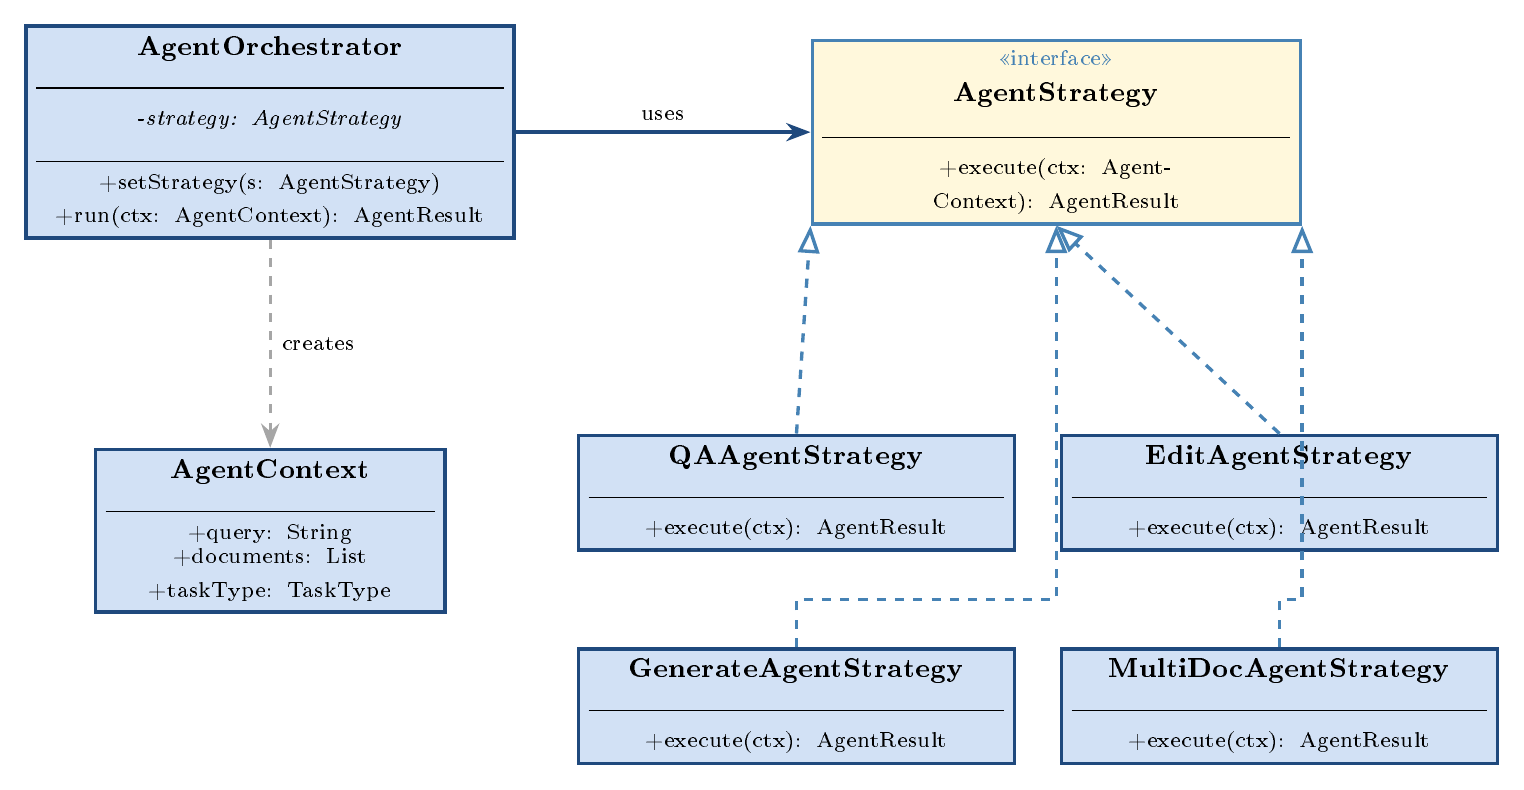
\includegraphics[width=0.88\textwidth]{uml_strategy_pattern.png}
  \caption{UML Class Diagram --- Strategy Pattern (Agent Orchestration)}
  \label{fig:uml_strategy_pattern}
\end{figure}

\paragraph{NFRs Addressed.}
\begin{itemize}[nosep]
    \item \textbf{Modifiability} --- new agent modes (e.g.\ a summarization agent) can be added
    without touching the orchestrator.
    \item \textbf{Performance} (NFR1) --- each strategy is optimized for its task class; the
    Q\&A strategy uses fast retrieval paths while the multi-document strategy uses batched
    retrieval.
    \item \textbf{Testability} --- each strategy can be unit-tested in isolation by injecting a
    mock \texttt{AgentContext}.
\end{itemize}

% ----------------------------------------------------------
\subsubsection{Pattern 2 --- Chain of Responsibility (LLM Request Pipeline)}
% ----------------------------------------------------------

\paragraph{Role in Architecture.}
The Chain of Responsibility pattern is instantiated in \textit{two} places in DocPilot:

\begin{enumerate}[nosep]
    \item \textbf{Model Fallback Chain (ModelGateway):} Handlers represent LLM providers in
    priority order. If the primary provider fails, the request propagates to the next handler
    until it is serviced or the chain is exhausted. This realizes Tactic~1 (Availability).

    \item \textbf{RAG Request Processing Pipeline:} The sequence of pipeline stages---Intent
    Resolution $\to$ Retrieval $\to$ Context Budgeting $\to$ Prompt Construction $\to$ LLM
    Call $\to$ Citation Grounding $\to$ Render---is modeled as a chain where each handler
    performs its transformation and passes the enriched context object to the next stage.
\end{enumerate}

\paragraph{Problem Solved.}
Without this pattern, the pipeline would be implemented as a monolithic function with deeply
nested logic, making it difficult to add, remove, or reorder stages (e.g.\ inserting a
re-ranking step between retrieval and context budgeting). The Chain of Responsibility makes each
stage independently replaceable and allows the pipeline to short-circuit (e.g.\ return a cached
response before reaching the LLM call stage).

\paragraph{Structural Description --- Model Fallback Chain.}

\begin{itemize}[nosep]
    \item \textbf{Abstract Handler:} \texttt{ModelProvider} --- declares \texttt{handle(request): Response}; holds a reference to \texttt{nextProvider}
    \item \textbf{Concrete Handlers:}
        \begin{itemize}[nosep]
            \item \texttt{OpenAIProvider} (primary)
            \item \texttt{AnthropicProvider} (first fallback)
            \item \texttt{GeminiProvider} (second fallback)
            \item \texttt{FallbackErrorHandler} (terminal handler; raises structured error)
        \end{itemize}
    \item \textbf{Client:} \texttt{ModelGateway} --- constructs and initiates the chain
\end{itemize}

\paragraph{Structural Description --- RAG Pipeline.}

\begin{itemize}[nosep]
    \item Each pipeline stage implements \texttt{PipelineHandler} with \texttt{process(ctx: PipelineContext): PipelineContext}
    \item Stages in order: \texttt{IntentResolver} $\to$ \texttt{Retriever} $\to$ \texttt{ContextBudgeter} $\to$ \texttt{PromptBuilder} $\to$ \texttt{LLMCaller} $\to$ \texttt{CitationGrounder} $\to$ \texttt{ResponseRenderer}
    \item Any stage may short-circuit by returning a completed \texttt{PipelineContext} without calling \texttt{next}
\end{itemize}

\begin{figure}[H]
  \centering
  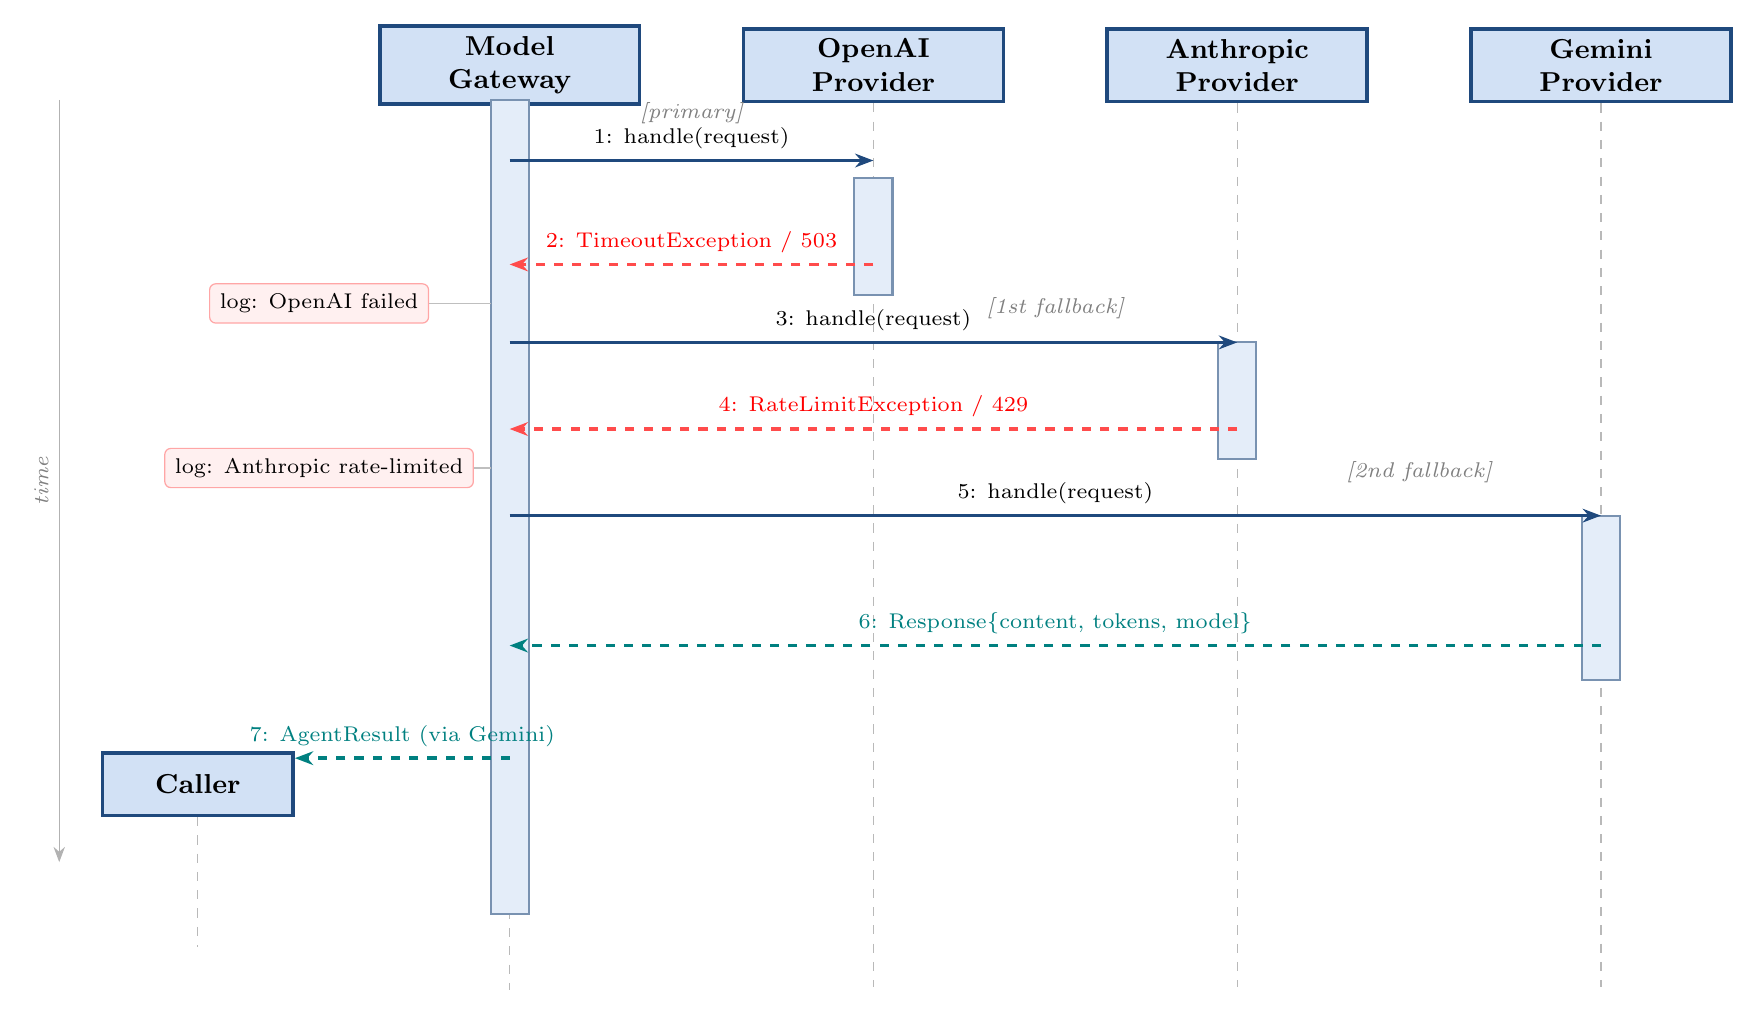
\includegraphics[width=0.88\textwidth]{uml_cor_sequence.png}
  \caption{UML Sequence Diagram --- Model Fallback Chain (Chain of Responsibility)}
  \label{fig:uml_cor_sequence}
\end{figure}

\begin{figure}[H]
  \centering
  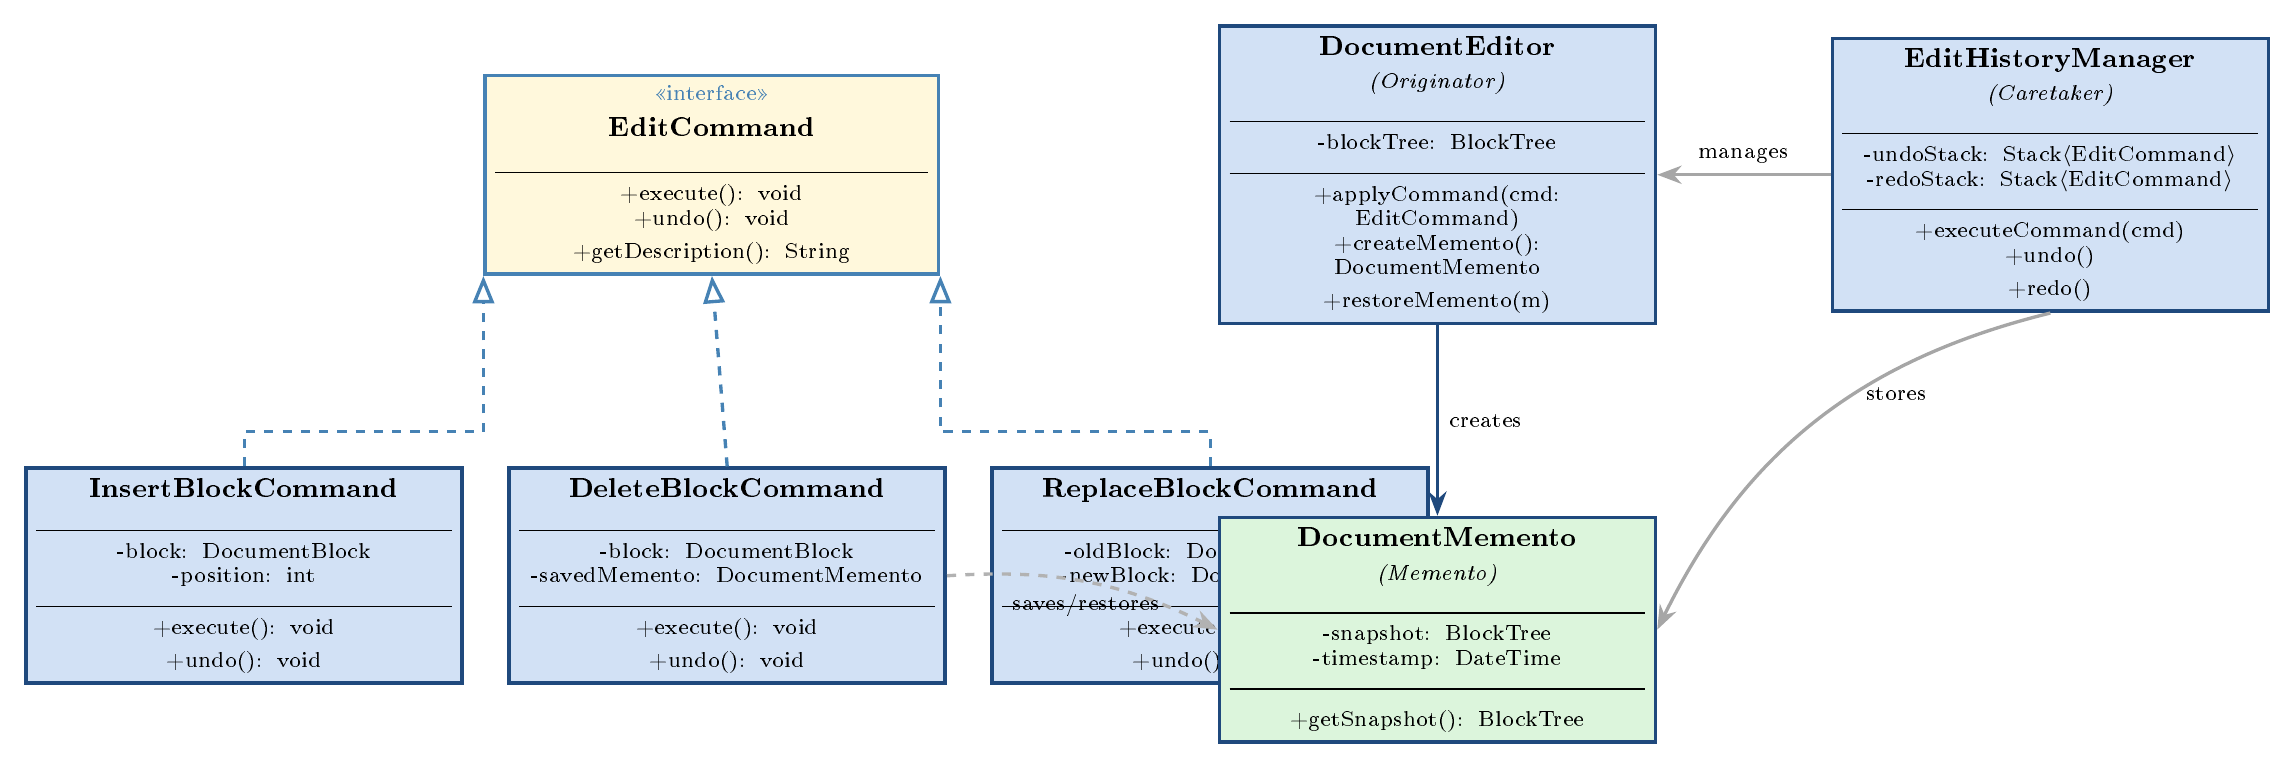
\includegraphics[width=0.88\textwidth]{uml_command_memento.png}
  \caption{UML Class Diagram --- Command + Memento Pattern (Reversible Edits)}
  \label{fig:uml_command_memento}
\end{figure}

\paragraph{NFRs Addressed.}
\begin{itemize}[nosep]
    \item \textbf{Availability} (NFR6) --- fallback chain ensures request is serviced even when
    primary or secondary providers fail.
    \item \textbf{Modifiability} --- new providers or pipeline stages can be inserted without
    modifying existing handlers.
    \item \textbf{Response Latency} (NFR1) --- the pipeline can short-circuit early (e.g.\ return
    a cached answer from the \texttt{Retriever} stage) reducing unnecessary LLM calls.
\end{itemize}

% ----------------------------------------------------------
\subsubsection{Companion Pattern --- Command + Memento (Reversible Edits)}
% ----------------------------------------------------------

\paragraph{Role in Architecture.}
Every AI-proposed edit is encapsulated as a \texttt{EditCommand} object (Command pattern) that
carries both the \texttt{execute()} and \texttt{undo()} operations. Before execution, the current
document state is saved as a \texttt{DocumentMemento} (Memento pattern). The
\texttt{EditHistoryManager} maintains an ordered stack of commands and mementos, enabling
multi-level undo and redo.

\paragraph{Structural Description.}
\begin{itemize}[nosep]
    \item \textbf{Command Interface:} \texttt{EditCommand} --- \texttt{execute()}, \texttt{undo()}
    \item \textbf{Concrete Commands:} \texttt{InsertBlockCommand}, \texttt{DeleteBlockCommand},
    \texttt{ReplaceBlockCommand}
    \item \textbf{Memento:} \texttt{DocumentMemento} --- immutable snapshot of the document block
    tree at a point in time
    \item \textbf{Originator:} \texttt{DocumentEditor} --- creates and restores mementos
    \item \textbf{Caretaker:} \texttt{EditHistoryManager} --- manages the undo/redo stacks
\end{itemize}

\paragraph{NFRs Addressed.}
\begin{itemize}[nosep]
    \item \textbf{Usability} --- full multi-level undo/redo with state restoration within 1 second.
    \item \textbf{Availability} --- reversibility prevents data loss from incorrect AI edits
    without requiring a full document reload.
    \item \textbf{Testability} --- each \texttt{EditCommand} can be unit-tested in isolation
    against a mock document state.
\end{itemize}

% ============================================================
\subsection{3.3 Tactics-to-NFR Mapping Summary}
% ============================================================

\begin{center}
\renewcommand{\arraystretch}{1.4}
\begin{tabularx}{\textwidth}{@{}L{4.5cm}L{2.8cm}L{2.8cm}L{4.5cm}@{}}
\toprule
\textbf{Tactic} & \textbf{Quality Attribute} & \textbf{NFR} & \textbf{Pattern Realization} \\
\midrule
Passive Redundancy / Spare & Availability & NFR6 & Chain of Responsibility (ModelGateway) \\
Limit Access / Manage Event Rate & Security + Availability & NFR1, NFR5 & Rate-limit middleware in ModelGateway \\
Dynamic Model Selection & Performance & NFR1, NFR5 & Strategy (ModelSelectionStrategy) \\
Separate Interface / Specialize Access & Testability & Pipeline coverage & Interface segregation + TEST\_MODE endpoints \\
Cancel/Undo + System Confirmation & Usability & Error recovery & Command + Memento \\
\bottomrule
\end{tabularx}
\end{center}

\end{document}